\section{}
% A washing machine produces disruptive noise during its spin cycle due to an uneven distribution 
% of clothes around its circumference. To reduce the noise, an engineering consulting firm has 
% proposed that the machine be mounted on spring isolators at each corner (four in total).
% The machine has a capacity of 10 kg of laundry, an unloaded mass of 450 kg, a drum diameter of 
% 0.50 m, and spin cycle speed of 955 rpm. To address the noise levels, the transmitted force should 
% be reduced by 75%. Assume vertical vibrations only and that 𝑐𝑒𝑓𝑓 is inherent to the system 
% (damping from the spring isolators are negligible).

A washing machine produces disruptive noise during its spin cycle due to an uneven distribution of clothes around its circumference. To reduce the noise, an engineering consulting firm has proposed that the machine be mounted on spring isolators at each corner (four in total). The machine has a capacity of 10 kg of laundry, an unloaded mass of 450 kg, a drum diameter of 0.50 m, and spin cycle speed of 955 rpm. To address the noise levels, the transmitted force should be reduced by 75\%. Assume vertical vibrations only and that $c_{\text{eff}}$ is inherent to the system (damping from the spring isolators are negligible).

% a) (5 pts) Determine the isolator spring constant needed to resolve the noise issue. Assume 
% that the system is 25% damped at full capacity (𝜁 = 0.25)
% b) After installing an appropriate set of spring isolators, it was found that a 0.3 kg wet hoodie 
% was spinning out of balance.
% i. (2.5 pts) Using the stiffness from part a), find the response amplitude due to this 
% imbalance during the spin cycle for the washing machine when it is fully loaded.
% ii. (2.5 pts) After removing the hoodie and resuming the same wash, a wet towel 
% with a mass of 0.5 kg began to spin out of balance. Determine the spring constants 
% needed to maintain the same amplitude as part i).

\begin{enumerate}[label=(\alph*)]
    \item (5 pts) Determine the isolator spring constant needed to resolve the noise issue. Assume that the system is 25\% damped at full capacity ($\zeta = 0.25$).
    \item After installing an appropriate set of spring isolators, it was found that a 0.3 kg wet hoodie was spinning out of balance.
    \begin{enumerate}[label=(\roman*)]
        \item (2.5 pts) Using the stiffness from part a), find the response amplitude due to this imbalance during the spin cycle for the washing machine when it is fully loaded.
        \item (2.5 pts) After removing the hoodie and resuming the same wash, a wet towel with a mass of 0.5 kg began to spin out of balance. Determine the spring constants needed to maintain the same amplitude as part i).
    \end{enumerate}
\end{enumerate}

\subsection*{Solution}
\subsection{}
This is an undamped SDOF spring damper system. The transmissibility is 
\begin{align*}
    \text{TR} &= \frac{\sqrt{1 + \left(2 \zeta \frac{\omega}{p}\right)^2}}{\sqrt{\left[1 - \left(\frac{\omega}{p}\right)^2\right]^2 + \left[2 \zeta \frac{\omega}{p}\right]^2}}
\end{align*}
Substituting $\text{TR} = 0.25$, $\zeta = 0.25$, $\omega = 955 \times \frac{2\pi}{60}$,
\begin{align*}
    0.25 &= \frac{\sqrt{1 + \left(2 \times 0.25 \times \frac{955 \times 2\pi/60}{p}\right)^2}}{\sqrt{\left[1 - \left(\frac{955 \times 2\pi/60}{p}\right)^2\right]^2 + \left[2 \times 0.25 \times \frac{955 \times 2\pi/60}{p}\right]^2}}
\end{align*}
Solving for $p$,
\begin{verbatim}
syms p real
eqn = 0.25 == sqrt(1+(2*0.25*955*2*pi/60/p)^2) / ...
sqrt((1-(955*2*pi/60/p)^2)^2+(2*0.25*955*2*pi/60/p)^2);
p = solve(eqn, p);
p = double(p)

p =
    -36.0438
    36.0438
\end{verbatim}
Therefore, the natural frequency is $36.0438$ rad/sec. The spring constant is then
\begin{align*}
    p &= \frac{k_{\text{eff}}}{m_{\text{eff}}} \\
    p &= \frac{4k}{m_{\text{eff}}} \\
    \implies k &= \frac{p^2 (m + \tilde{m})}{4} \\
    &= \frac{(36.0438)^2(450 + 10)}{4} \\
    &= \boxed{1.494 \times 10^5 \text{ N/m}}
\end{align*}

\subsection{}
\subsubsection{}
The system now is a damped rotating imbalance where $M = 460$, $\tilde{m} = 0.3$.

The response ampltitude curve is shown in the figure
\begin{figure}[h]
    \centering
    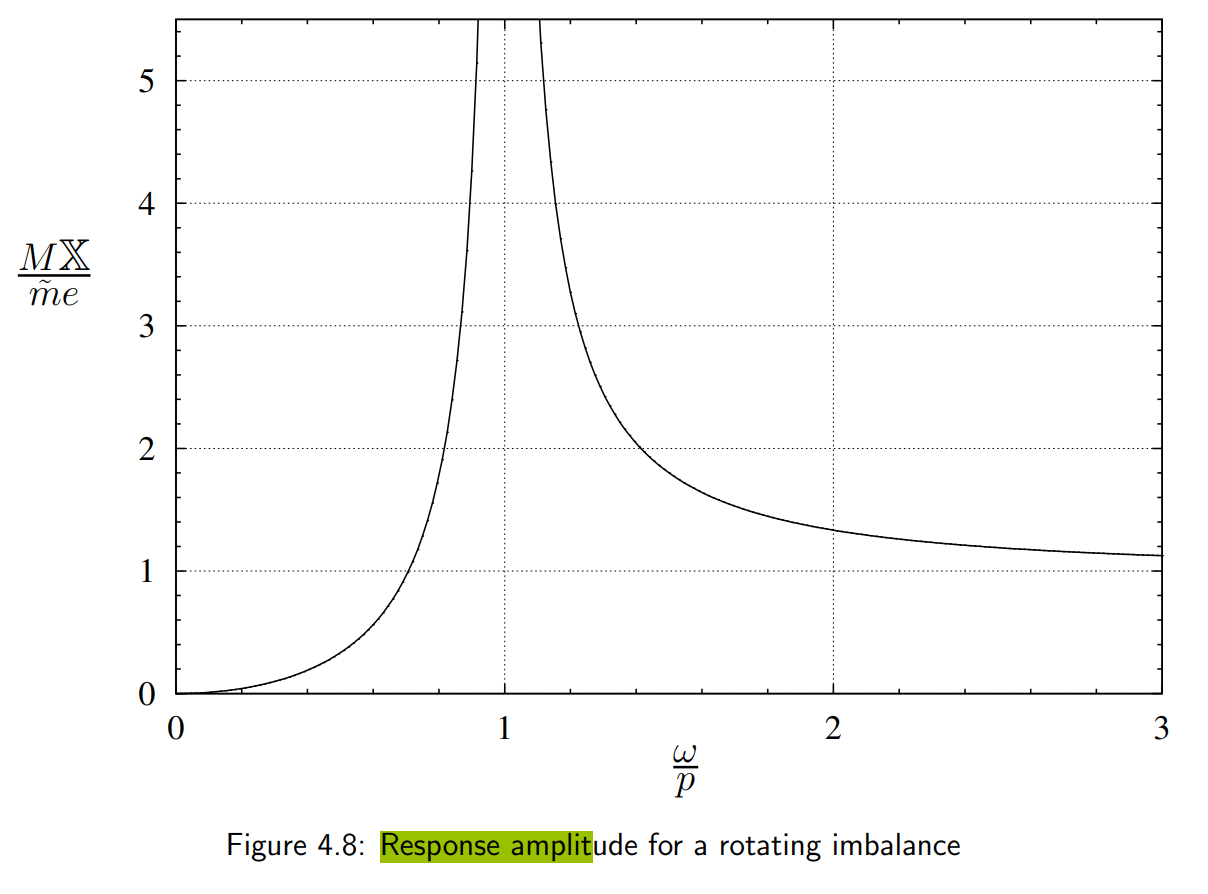
\includegraphics[width=0.5\textwidth]{Questions/Figures/q4 response ampltiude.png}
\end{figure}
\FloatBarrier
The damping ratio is the same since effective mass has not changed.
Then the response amplitude
\begin{align*}
    \frac{M \mathbb{X}}{\tilde{m} e} &= \frac{\left(\frac{\omega}{p}\right)^2}{\sqrt{\left[1 - \left(\frac{\omega}{p}\right)^2\right]^2 + \left[2 \zeta \frac{\omega}{p}\right]^2}} \\
    &= \frac{\left(\frac{955 \times 2\pi/60}{36.0438}\right)^2}{\sqrt{\left[1 - \left(\frac{955 \times 2\pi/60}{36.0438}\right)^2\right]^2 + \left[2 \times 0.25 \times \frac{955 \times 2\pi/60}{36.0438}\right]^2}} \\
    &= \boxed{1.1254}
\end{align*}
the amplitude is therefore,
\begin{align*}
    \mathbb{X} &= \frac{1.1254 \times 0.3 \times 0.25}{460} \\
    &= \boxed{0.00018349 \text{ m}}
\end{align*}

\subsubsection{}
The new system has $M = 459.7$, $\tilde{m} = 0.5$. Damping ratio needs to be recalcualted since the effective mass has changed. Since $c_{\text{eff}}$ is inherent to the system, we solve for it using values from part a),
\begin{align*}
    \zeta_{\text{a}} &= \frac{c_{\text{eff}}}{2 m_{\text{eff}} p} \\
    \implies c_{\text{eff}} &= 2 \zeta_{\text{a}} m_{\text{eff}} p \\
    &= 2 \times 0.25 \times (460) \times 36.0438 \\
    &= 8290.074 \text{ Ns/m}
\end{align*}
Then the new damping ratio is
\begin{align*}
    \zeta &= \frac{8290.074}{2(459.7)36.0438} \\
    &= 0.25016314988
\end{align*}

The formula for response amplitude is 
\begin{align*}
    \frac{M \mathbb{X}}{\tilde{m} e} &\overset{\text{set}}{=} \frac{459.7 \cdot 0.00018349}{0.5 \cdot 0.25} = 0.674802824 \\
    &= \frac{\left(\frac{\omega}{p}\right)^2}{\sqrt{\left[1 - \left(\frac{\omega}{p}\right)^2\right]^2 + \left[2 \zeta \frac{\omega}{p}\right]^2}} \\
    &= \frac{\left(\frac{955 \times 2\pi/60}{p}\right)^2}{\sqrt{\left[1 - \left(\frac{955 \times 2\pi/60}{p}\right)^2\right]^2 + \left[2 \cdot 0.25016314988 \cdot \frac{955 \times 2\pi/60}{p}\right]^2}}
\end{align*}
where we solve for $p$,
\begin{verbatim}
syms p
eqn = 0.674802824 == (955*2*pi/60/p)^2/sqrt((1-(955*2*pi/60/p)^2)^2 ...
+(2*0.25016314988*955*2*pi/60/p)^2);
p = solve(eqn, p);
p = double(p)

p =
    -150.8534
     150.8534 
\end{verbatim}
Therefore, the natural frequency is $150.8534$ rad/sec. The spring constant is then
\begin{align*}
    k &= p^2(M+ \tilde{m})/4 \\
    &= (150.8534)^2(459.7 + 0.5)/4 \\
    &= \boxed{2.618 \times 10^6 \text{ N/m}}
\end{align*}